\subsection{Adquisición de Contexto}
\label{subsec:Prop_Adquisicion}

En esta capa se obtienen los datos que serán analizados para encontrar el contexto de la entidad más importante de la propuesta, el usuario. Según Perera et al.\cite{Perera2014} un componente de adquisición debe tener en cuenta aspectos como la frecuencia de obtención y tipo de sensor, en esta arquitectura \textbf{\textit{(i)}} los datos de contexto se obtienen de forma periódica y \textbf{\textit{(ii)}} las fuentes de contexto son variadas. Las fuentes de información de esta propuesta se dividen en 3 grupos:
\begin{itemize}
    \item \textbf{Sensores de Entidades}: Esta categoría sigue la definición de entidad de Dey et al.\cite{Dey2001}, esto es de gran importancia teniendo en cuenta que en la actualidad un auto, una casa, un teléfono o una persona pueden llevar sensores que generan información acerca de su condición y la de su entorno. Es posible entonces combinar información contextual de un vehículo y su conductor (CITA TRABAJO CONTEXTO/RAZONAMIENTO) o de un anciano con su hogar (CITA CONTEXTO/APLICACIÓN).
    \item \textbf{Contenido Multimedia}: Representa el aporte de este trabajo y sigue los lineamientos presentados en las secciones \ref{sec:MT_ContenidosMultimedia} y \ref{sec:Prop_MultimediaContext}. Parte de la hipótesis de que los contenidos que producen los usuarios en diferentes situaciones almacenan información contextual de utilidad para definir las situaciones de una persona en diferentes momentos. Información de contexto de naturaleza social como las personas con las que se compartió un momento, o dependiente de un campo de aplicación en específico como los cantos de algunas aves cuando se realizaba una exploración en campo permiten que una aplicación modifique su funcionamiento y facilite las actividades que este debe realizar.
    \item \textbf{Datos Externos}: Este grupo corresponde a la descripción de Sensores Lógicos presentados por \cite{Perera2014}, con este grupo se asegura el uso de información proveniente de servicios web que puede modificar o complementar el contexto de un usuario. Un ejemplo es el registro del clima en el lugar de interés de un turista, o el listado de eventos sociales que se desarrollan un fin de semana (incluyendo costos y horarios).
\end{itemize}

\subsection{Pre-procesamiento de los datos}
\label{subsubsec:Prop_Adqui_PrePro}

De acuerdo al ciclo de vida de los sistemas sensibles al contexto es necesario realizar procesos de filtrado de información, este proceso asegura la eliminación de datos fuera de orden, la unión de mediciones ocurridas en periodos iguales de tiempo y también la identificación del contexto de bajo nivel por medio de la identificación de actividades de forma automática.
El pre-procesamiento de los datos dependerá de las tecnologías pertinentes al sistema al desarrollar, en este trabajo se propone una arquitectura de tres capas con las siguientes características, Fig  \ref{fig:Diagrama_preprocesa}:
\textbf{\textit{(i)}} fuentes de contexto, 
\textbf{\textit{(ii)}} tipos de dato producidos por las fuentes de contexto,
\textbf{\textit{(iii)}} algoritmos de procesamiento,
\textbf{\textit{(iv)}} uso de estándares para el etiquetado de actividades reconocidas.
\begin{figure}[ht]
    \centering%
    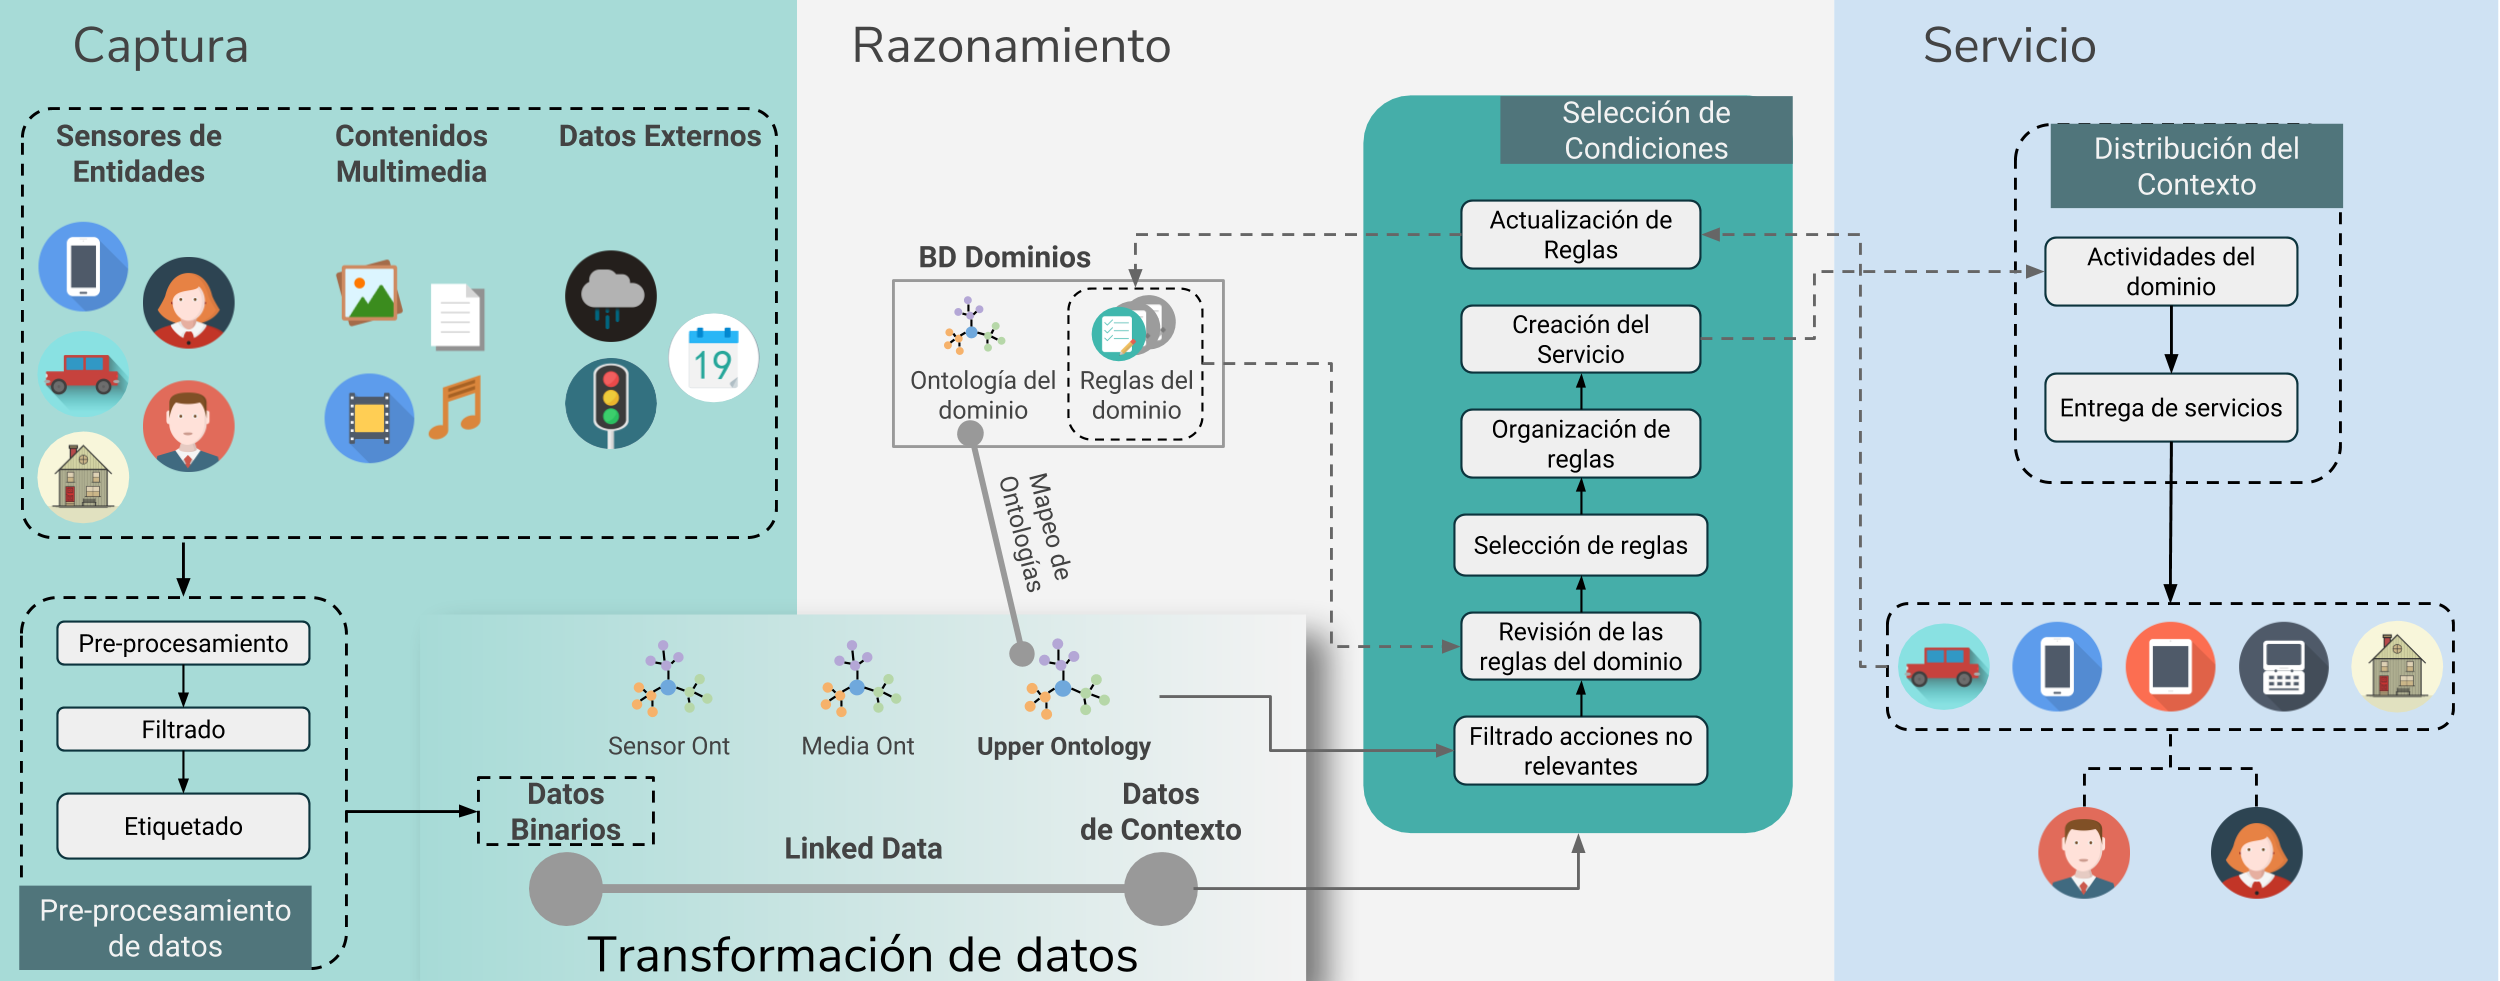
\includegraphics[width=\textwidth]{https://docs.google.com/drawings/d/1pNA08-j5f8h--PJIRJZafjfwxJ1rQbj0zHwOFvc57LA/edit     Cap3/Images/Diagrama_Contexto_v2}%
    \caption{Arquitectura de contexto MCARS.} \label{fig:Diagrama_preprocesa}
\end{figure}
    


sigue los parámetros presentados en la Arquitectura General \ref{sec:Prop_Arquitectura} (O CITAR EL COMPONENTE DE LA ARQUITECTURA GENERAL).